\section{Metodologie}

Per avviare la progettazione dell'ontologia OFFF, è stato analizzato il contenuto nutrizionale incentrato sul consumatore da fast food (quali sono McDonalds, Dairy Queen, Chick Fil-A, Wendy's, Taco Bell, Arby's, Blimpie, Carl's Jr, Checkers\& Rally's, Church's, Jack in the Box, Jollibee, Popeye's, Raising Cane's, White Castle e Panda Express), i loro siti Web forniscono dati nutrizionali. 
E' stata quindi ideata la struttura dei metadati partendo dalle fonti, si sono identificati i concetti principali con le relazioni tra di loro sfruttando come guida l'etichetta nutrizionale di \emph{Food and Drug Administration}. 
Questa attività ha prodotto l'astrazione del metalivello dell'ontologia (Vedi Fig.\ref{fig:ontology}). 
\begin{figure}[H]
    \centering
    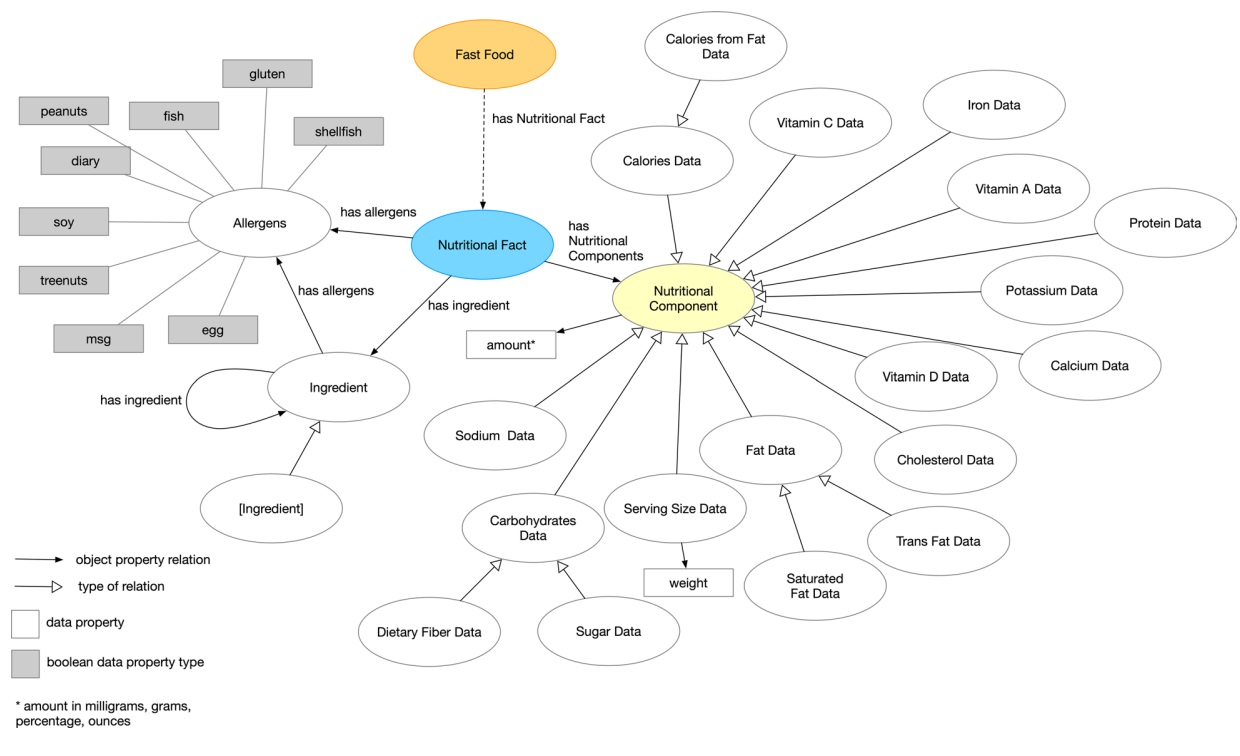
\includegraphics[width=\textwidth]{res/WS_01_Ontology_Meta_Level.jpg}
    \caption{Meta-livello dell'ontologia di OFFF che mostra la rappresentazione del concetto di Fatto Nutrizionale e la sua relazione con il concetto di Fast Food. Il nodo giallo scuro indica sottoclassi aggiuntive}
     \label{fig:ontology}
\end{figure}
Il concetto centrale del metalivello di questa ontologia è il Fatto Nutrizionale. Questo concetto contiene relazioni con la componente nutrizionale, l'ingrediente e gli allergeni. Il meta-livello dell'ontologia è stato creato utilizzando Protégé.
Successivamente, è stato valutato la veridicità della struttura del meta-livello dell'ontologia utilizzando Hootation, una libreria di software per la generazione di linguaggio naturale per ontologie. 
I valutatori dell'albero (CO, GX e CT) hanno esaminato in modo indipendente le dichiarazioni in lingua naturale tradotte (Burrito\_Pollo\_Sminuzzato $\subset$ Burrito tradotto in "ogni burrito di pollo sminuzzato è un burrito") che esprime ogni assioma logico codificato nell'ontologia. 
A ciascun valutatore è stato fornito un foglio di calcolo con gli assiomi tradotti e gli è stato chiesto di etichettare le affermazioni: "Sì" se l'assioma logico è accurato, "No" se l'assioma non è accurato o "X" se il valutatore non era sicuro.

\subsection{Componenti nutrizionali}
La Componente nutrizionale ha diverse sottoclassi che alludono a vari dati nutrizionali trovati sulle etichette degli alimenti: proteine, colesterolo, grassi, minerali, ecc. 

Essenzialmente, Componente nutrizionale descrive la quantità di nutrienti che un particolare alimento possiede. È espresso attraverso una proprietà dei dati di \emph{Amount} (in milligrammi, grammi, once, ecc.). 
Indichiamo anche quantità di vitamine e minerali contenuti in un alimento: ferro, vitamina A, calcio, potassio, ecc. È stato limitato alle vitamine e ai minerali che vengono divulgati dalle fonti online.

\subsection{Allergeni}
Il fatto nutrizionale include informazioni sugli allergeni, essi sono rappresentati come \emph{Fatto nutrizionale → ha allergeni → allergeni}. Il concetto di \emph{Allergens} ha diversi tipi di dati booleani per alterare l'alimento per il contenuto di allergeni (soia, msg, uova, diario, ecc.).

\subsection{Ingredienti}
Le informazioni sugli ingredienti per i prodotti alimentari sono rappresentate nell'ontologia come \emph{Fatti nutrizionali → contiene ingredienti → Ingrediente}. La classe \emph{Ingredient} copre qualsiasi componente elencato dai dati nutrizionali come pane, uova, sciroppo di mais, caffeina, ecc. 
Questo concetto ha anche una relazione autodiretta, \emph{"ha ingredienti"} se determinati ingredienti contenevano altri ingredienti. Ad esempio, il pane può contenere latte e uova (es. pane → contiene ingredienti → latte e pane → contiene ingredienti → uovo). 
Infine, il concetto di ingrediente ha un collegamento con gli allergeni che utilizzano allergeni. Se un alimento contiene latte, può essere indicato con una reazione allergica.

\subsection{Concetto di fast food}
Il meta-livello, descritto sopra, funge da struttura per le informazioni nutrizionali dei consumatori. Per i prodotti da fast food, è stata creata una classe chiamata \emph{Fast Food} che è sottoclasse di un'entità \emph{Food}. Questo concetto è usato per descrivere i tipi di fast food nella maggior parte dei fast food. 
Si è anche incluso un concetto chiamato Fast Food Restaurant (collegato a Fast Food tramite offerto da) che è una classe discendente di Agent, seguendo come altre ontologie come PROV-O (Provenance ontologia) e FOAF (Friend of a friendontology) che rappresentano organizzazioni (Agente $>$ Organizzazione $>$ Affari). 
Sulla base della selezione limitata di fast food, si sono identificate 10 categorie di fast food di base (vedi Fig.\ref{fig:fastFood}). Fast Food è collegato a \emph{Nutritional Fact} con la proprietà oggetto di ha Nutritional Fact per associare gli alimenti da fast food ai dati nutrizionali.

\begin{figure}[H]
    \centering
    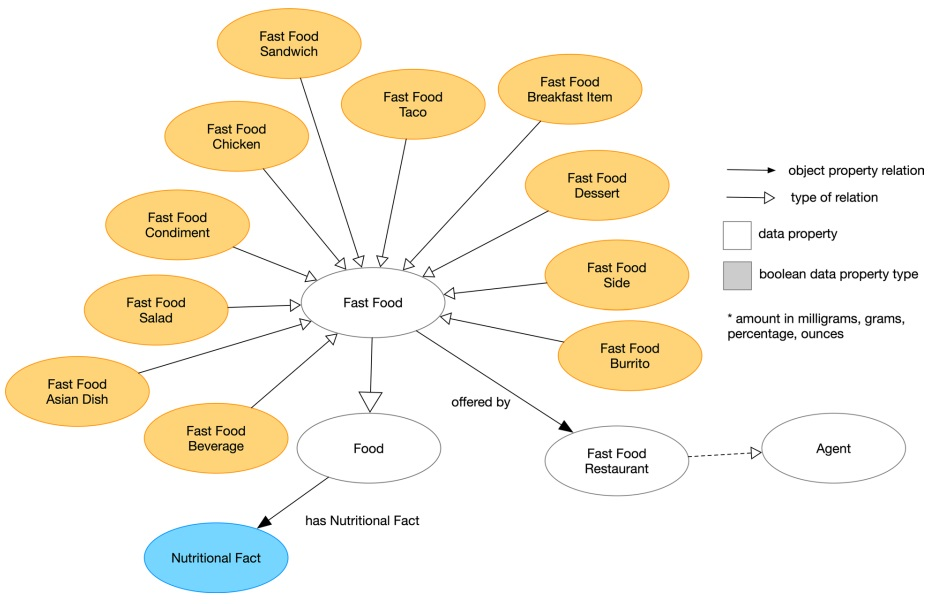
\includegraphics[width=\textwidth]{res/WS_02_Fast_Food_Category.jpg}
    \caption{Meta-livello dettagliato dell'ontologia di OFFF che mostra le sottocategorie del fast food. Il nodo giallo scuro indica sottoclassi aggiuntive}
     \label{fig:fastFood}
\end{figure}

\subsection{Instance Data Model}
I dati nutrizionali dei menu dei fast food sono stati rappresentati come esempi unici per l'ontologia. I sopraccitati fast food hanno dati nutrizionali sul sito Web. Sono stati trasferiti i dati dalle sorgenti a un foglio di calcolo per l'importazione. Sono stati utilizzato \emph{Protégéplugin} e \emph{Cellfe}, per eseguire l'importazione di massa dei dati sugli alimenti. 
Si è creato una serie di regole di importazione personalizzate per Cellfe per normalizzare e aggiungere i dati all'ontologia. La figura \ref{fig:OntologyInstance} visualizza i dati di un'istanza di esempio dall'ontologia dei fatti del fast food. L'elemento \emph{Tefood} istanzia il tipo di fast food. Nell'esempio sopra, Iced Cofee McDonald's (Small) è un esempio di Cofee che è un tipo di bevanda. Questo elemento di dati si collega ad altre informazioni nutrizionali e sugli allergeni utilizzando \emph{hasNutritionalInfo} e \emph{hasAllergens}, come mostrato in Fig. \ref{fig:OntologyInstance}. 

\begin{figure}[H]
    \centering
    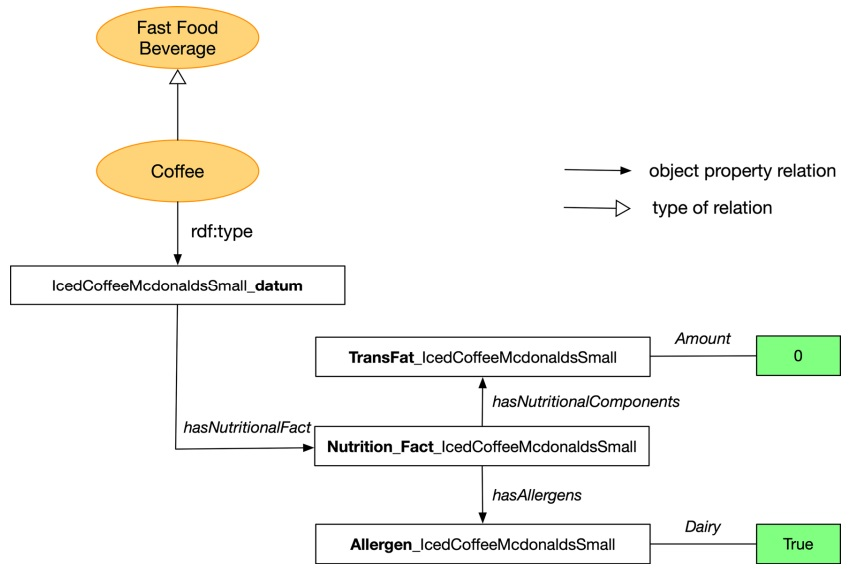
\includegraphics[width=\textwidth]{res/WS_03_Ontology_Instance_Example.jpg}
    \caption{Visualizzazione di un'istanza campione dall'ontologia dei fatti di fast food. Il suffisso e il prefisso sono in grassetto per evidenziare il tipo di informazioni sull'istanza}
     \label{fig:OntologyInstance}
\end{figure}

\subsection{Arricchimento da comuni domande nutrizionali}
In questa fase sono state raccolte le domande dei consumatori facendo ricerche web utilizzando come chiave di ricerca frasi come "Domande frequenti \\sull'alimentazione" e "Domande più comuni sull'alimentazione". Sono state selezionate sei fonti, ciascuna delle quali elencava le domande frequenti relative alla nutrizione a cui hanno risposto nutrizionisti registrati o dietologi registrati. Le fonti hanno prodotto 41 domande che sono state ristrette per includere 19 domande che sono state utilizzate per espandere l'ontologia.
La tabella \ref{fig:Questions} elenca le 19 domande finali relative ai risultati associati a zucchero, sodio e grassi.
La figura \ref{fig:ConcettiAggiuntivi} modella i concetti aggiuntivi e le relazioni con OFFF. Ciò include l'aggiunta di due nuovi concetti: risultati sulla salute e qualità della dieta che sono stati estesi attraverso il concetto esistente di componente nutrizionale.
Questo includeva anche ulteriori sottoclassi dei suddetti concetti, tutte mostrate in Fig. \ref{fig:ConcettiAggiuntivi}. Queste derivazioni sono state codificate nell'ontologia dei fatti del fast food utilizzando Protégé.

\begin{figure}[H]
    \centering
    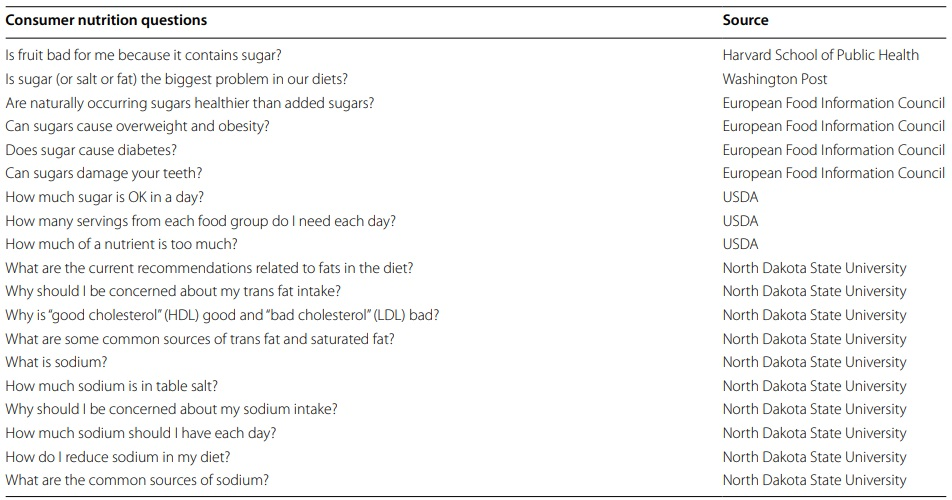
\includegraphics[width=\textwidth]{res/WS_04_Questions.jpg}
    \caption{19 Domande dei consumatori utilizzate per espandere l'ontologia dei fatti sui fast food}
     \label{fig:Questions}
\end{figure}

\begin{figure}[H]
    \centering
    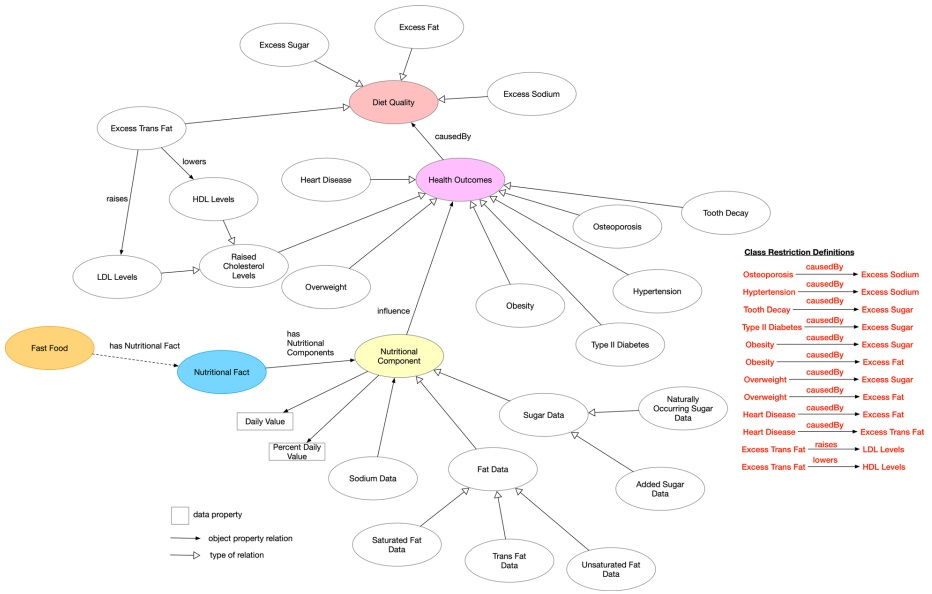
\includegraphics[width=\textwidth]{res/WS_05_Concetti_Aggiuntivi.jpg}
    \caption{Una mappa concettuale che delinea i concetti aggiuntivi derivati dalle domande sull'alimentazione dei consumatori. A fini di leggibilità, sono elencate le definizioni delle restrizioni di classe}
     \label{fig:ConcettiAggiuntivi}
\end{figure}

\subsubsection{Risultati sulla salute}
Il concetto di \emph{Health Outcomes} è costituito da sottoclassi che rappresentano vari esiti negativi per la salute associati alla qualità della dieta. Questi risultati includono obesità, carie, ipertensione, diabete di tipo 2, osteoporosi, sovrappeso, malattie cardiache e livelli di colesterolo elevati. I risultati sulla salute sono collegati all'influenza dei componenti nutrizionali.

\subsubsection{Qualità della dieta}
Il concetto di qualità della dieta consiste in sottoclassi che rappresentano attributi identificati come fattori che contribuiscono a una dieta di scarsa qualità: eccesso di grassi saturi, grasso in eccesso, zucchero in eccesso e sodio in eccesso. Ciascuna sottoclasse è collegata a una sottoclasse del concetto Health Outcomes utilizzando la proprietà dell'oggetto \emph{causedBy}, \emph{raises} e \emph{lowers}. La Figura \ref{fig:ConcettiAggiuntivi} elenca le restrizioni di classe per queste sottoclassi.

\subsubsection{Valore giornaliero e valore giornaliero \%}
La proprietà dei dati \emph{Daily Value} esprime il valore giornaliero raccomandato di un componente nutrizionale. \emph{NutritionalComponent} viene esteso utilizzando la proprietà dei dati Daily Value (valore intero positivo). Allo stesso modo, si è incluso anche la percentuale del valore giornaliero (percentuale del valore giornaliero) come tipo di valore decimale.